% ADD/REMOVE THE 'answers' OPTION TO INCLUDE/SUPPRESS SOLUTIONS
% \documentclass[11pt,addpoints]{exam}
\documentclass[11pt,addpoints,answers]{exam}

\newcommand{\hwnum}{7}
\newcommand{\duedate}{March 19}

% In order to compile this file you will need to get 'header.tex'
% and make the line below point to the appropriate file path
\input{header}
\usetikzlibrary{positioning}

\newcommand{\ptimemap}{\leq_p}
\newcommand{\tred}{\leq_T}

\ifprintanswers
\hwslnheader   % header for solutions
\else
\hwheader   % header for homework
\fi

\begin{document}



\begin{questions}

  \question[10] \textbf{Self assessment.} \nopagebreak
  
  Carefully read and understand the posted solutions to the \textbf{midterm exam}. Identify \textbf{one problem from the list below} for which your own solution has the most room for improvement (e.g., has unsound reasoning, doesn’t show what was required, could be significantly clearer or better organized, etc.).
  \begin{itemize}
      \item Q10 Chaotic Potential
      \item Q13 Greedy Cat Photographing
      \item Q14 DFA Impossibility
      \item Q15 SpongeBob vs Squidward
      \item Q16 Machine Disagreement
  \end{itemize}
  Copy or screenshot your solution, then in a few sentences, explain what was deficient and how it could be fixed.

  (Alternatively, if you think one of your solutions is significantly \emph{better} than the posted one, copy it here and explain why you think it is better.)

  If you didn't take the exam, review \href{https://drive.google.com/file/d/1cky3dbWYKLzPwVmNGsx5TeEW42zbEdBa/view?usp=drive_link}{this solution} by GPT 4o instead (pick one problem and explain the room for improvement). 

  \begin{solution} 
  My solution for Q14 of the midterm is as follows:
  \begin{center}
    \includegraphics[width=0.8\linewidth]{q14midterm.png}
  \end{center}
  My solution was fundamentally deficient because of the way that I approached the problem. Instead of using the definition of a DFA, and taking advantage of the fact that a DFA has a finite amount of states with the pigeonhole principle, I tried to define a contradictory turing machine that would accept the language, and then show that the language was turing rediculable to $L_{ACC}$. This was a convoluted approach, but I did have the right idea to contradict a supposed DFA that decides tha language. I could have fixed this by using the definition of a DFA, and showing that the language is not regular by the pigeonhole principle.
  \end{solution}

\question \textbf{Understanding \P, \NP, and \NP-hardness.}
\begin{parts}
  \part [4] Prove that all efficiently decidable languages are efficiently verifiable. In other words, show that every language in $\P$ has an efficient verifier. 
  
  \begin{solution}
  Since every language in \(\P\) has a polynomial-time decider \(D\), construct a verifier \(V\) that, on input \((x,y)\), simply ignores \(y\) and simulates \(D\) on \(x\). If \(D\) accepts, then \(V\) accepts; otherwise, \(V\) rejects. The simulation runs in polynomial time, so all languages in \(\P\) admit efficient verifiers.
  \end{solution}

  \part[4] Prove that every language in $\NP$ is decidable. In other words, show that every language in $\NP$ has a decider. 

  \begin{solution}
  Let \(L\in\NP\). By definition, there is a nondeterministic polynomial-time Turing machine \(N\) deciding \(L\). To decide \(L\) deterministically, on input \(x\), systematically simulate every nondeterministic branch of \(N\) on \(x\). Since each branch runs in polynomial time, this procedure halts on every branch and accepts exactly when \(x\in L\). Thus, \(L\) is decidable.
  \end{solution}

  \part [4] Prove or disprove: All \NP-hard languages are decidable. 

  (A disproof would consist of an \NP-hard language that is also undecidable.) 

  \begin{solution}
  Disprove; define
  \[
  L \;=\; \{\,\varphi \mid \varphi\in \text{3SAT}\}\;\cup\;\{\,\langle M\rangle \mid M\text{ halts on the empty input}\}.
  \]
  \textbf{1. Reduction:} Given an instance \(\varphi\) of 3SAT, let \(f(\varphi)=\varphi\).\\
  \textbf{2. Polynomial Time:} This is the identity function; polynomial time.\\
  \textbf{3. Correctness:} 
  \begin{itemize}
  \item (\(\Rightarrow\)) If \(\varphi\) is satisfiable, then \(\varphi \in L\), so \(f(\varphi)\in L\).
  \item (\(\Leftarrow\)) If \(f(\varphi)=\varphi\in L\), then \(\varphi\) must be a satisfiable 3SAT instance. 
  \end{itemize}
  Hence 3SAT \(\leq_p\) \(L\), so \(L\) is \NP-hard. However, deciding \(L\) requires solving the Halting Problem, so \(L\) is not decidable. Therefore, not all \NP-hard languages are decidable.
  \end{solution}
    
\end{parts}

\pagebreak
  \question \textbf{Verifying $\Upsilon$'s verifiers.} \label{Upsilon-verifiers}

    \emph{We highly recommend you to read the \href{https://eecs376.github.io/notes/complexity.html\#discussion-of-completeness-and-soundness}{Discussion of Completeness and Soundness} and \href{https://eecs376.github.io/notes/complexity.html\#discussion-of-efficiency}{Discussion of Efficiency} sections before attempting the following problem.}

    Recall that a \emph{multiset} $S$ is just like a set, but it can have duplicate elements. A submultiset $S^* \subseteq S$ also can have duplicate elements, as long as it does not have more copies of an particular element than $S$ does. 
    
    Consider the following language
    \newcommand{\SubsetSum}{\textsc{SubsetSum}}
    \[ 
        \SubsetSum = \set{(S, k) : S \text{ is a \emph{multiset} of integers $\geq 0$, and } \exists\; S' \subseteq S \text{ such that } \sum_{s \in S'} s = k}.
    \]

  \begin{parts}
      \part [4] Professor $\Upsilon$ claims that $\SubsetSum \in \NP$, and presents the following verifier: 
      \vspace{-10pt}
    \begin{center}
      \begin{minipage}{0.9\linewidth}
        \begin{algorithm}[H]
       \begin{algorithmic}[1]
      \Require{A multiset of nonnegative integers $S = \set{s_1, s_2, \ldots, s_n}$, an integer $k$, and \emph{a multiset of nonnegative integers} $C = \set{c_1, c_2, \ldots, c_m}$}
         \Function{VerifierA}{$S, k, C$}
         \If{$m > n$} \textbf{reject} \Comment{$C$ can't be a submultiset of $S$ in this case} \EndIf 
         \State $sum \gets 0$
         \For{$c \in C$} \Comment{iterate over elements (integers) in $C$}
         \If{$c \notin S$} \textbf{reject} 
         \Else { $sum \gets sum + c$}
         \EndIf
         \EndFor
         \If {$sum = k$} \textbf{accept} \EndIf
         \State \textbf{reject}
         \EndFunction
       \end{algorithmic}
     \end{algorithm}  
     \end{minipage}
     \end{center}
    \begin{quote}
        \textbf{Correctness:} For correctness,
        \begin{align*}
            (S,k) \in \SubsetSum &\iff \text{there exists a submultiset $C \subseteq S$ s.t. $\sum_{c \in C} c = k$} \\
            & \iff \textsc{VerifierA}(S,k,C) \text{ accepts}
        \end{align*}
      
        \textbf{Runtime:} After ruling out the possibility that $m > n$ in line 2, the for loop will iterate over at most $n$ elements, while other lines take constant time, the overall runtime is $O(n)$, which is polynomial with respect to the input size. 
    \end{quote}

    Explain why \textsc{VerifierA} does not show that $\SubsetSum \in \NP$. You may use an example to support your reasoning. You do not have to fix the verifier, though it is a good exercise. 

    \begin{solution} 
    \textsc{VerifierA} does not ensure that \(C\) is a valid submultiset of \(S\). Line 6 only checks whether each \(c \in C\) appears in \(S\), not whether the total number of occurrences of each integer in \(C\) exceeds its count in \(S\). If \(S = \{1,1\}\) and \(C = \{1,1,1\}\), line 6 verifies each \(1\) in \(C\) independently and never catches that \(C\) has too many \(1\text{'s}\). This failure to enforce correct repeats allows invalid certificates to be accepted, so \textsc{VerifierA} does not establish \(\SubsetSum \in \NP\).
    \end{solution}

      
      \part [4] $\Upsilon$ realizes their mistake and gives you another verifier, which takes a \emph{collection} of nonnegative integers \emph{multisets} as certificate (these multisets may or may not be submultisets of $S$) as follows.
      \vspace{-10pt}
    \begin{center}
      \begin{minipage}{0.9\linewidth}
        \begin{algorithm}[H]
       \begin{algorithmic}[1]
      \Require{A multiset of nonnegative integers $S = \set{s_1, s_2, \ldots, s_n}$, an integer $k$, and \emph{a collection of nonnegative integers multisets} $C = \set{C_1, C_2, \ldots, C_m}$}
         \Function{VerifierB}{$S, k, C$}
         \For{$C_i \in C$} \Comment{Iterate over multisets in $C$}
            \State Confirm that $C_i \subseteq S$
            \If {$\sum_{c \in C_i} = k$} \textbf{accept} \EndIf
         \EndFor
         \State \textbf{reject}
         \EndFunction
       \end{algorithmic}
     \end{algorithm}  
     \end{minipage}
     \end{center}

    \begin{quote}
        \textbf{Correctness:} For correctness,
        \begin{align*}
            (S,k) \in \SubsetSum &\iff \text{there exists a submultiset $C_i \subseteq S$ s.t. $\sum_{c \in C_i} c = k$} \\
            & \iff \text{there exists a collection $C$ that contains $C_i$}\\
            & \iff \textsc{VerifierB}(S,k,C) \text{ accepts}
        \end{align*}
      
        \textbf{Runtime:} In line 4, since $C_i$ is confirmed to be a submultiset of~$S$, $|C_i| \leq n$ and hence summing all items takes $O(n)$. Since there are $m$ sets in $C$, the overall runtime is $O(mn)$, which is polynomial with respect to the input size. 
    \end{quote}

      Explain why \textsc{VerifierB} does not show that $\SubsetSum \in \NP$. You may use an example to support your reasoning. You do not have to fix the verifier, though it is a good exercise. 

      \begin{solution}
      \textsc{VerifierB} takes a ``collection of submultisets'' as the certificate without restricting its size to be polynomial in \(\abs{S}\). Since there can be exponentially many submultisets in such a collection, the run time \(\text{(in terms of \(\abs{S}\) alone)}\) can become unbounded. For example, given \(S=\{1,2,\dots,n\}\), a certificate could include all \(2^n\) possible submultisets of \(S\). Even though each submultiset can be checked in polynomial time, the total number of submultisets makes verification exponential in \(\abs{S}\). Because the runtime must be polynomial in the size of the \emph{original input} to show \(\SubsetSum\in\NP\), \textsc{VerifierB} fails to establish membership in \(\NP\).
      \end{solution}

      \part [4] Frustrated by $\Upsilon$'s mistakes, Lambda presents the following verifier:
      \vspace{-10pt}
    \begin{center}
    \begin{minipage}{0.9\linewidth}
      \begin{algorithm}[H]
      \begin{algorithmic}[1]
    \Require{A multiset of nonnegative integers $S = \set{s_1, s_2, \ldots, s_n}$, an integer $k$, and \emph{an array of bits} $C[1,\ldots,n]$}
        \Function{VerifierC}{$S, k, C$}
          \State $sum \gets 0$
          \For {$i = 1, \ldots, n$}
              \If {$C[i] = 1$} $sum \gets sum + s_i$ \EndIf
          \EndFor
        \If {$sum = k$} \textbf{accept} \EndIf
        \State \textbf{reject}
        \EndFunction
      \end{algorithmic}
    \end{algorithm}  
    \end{minipage}
    \end{center}

    $\Upsilon$ claims that Lambda's verifier is incorrect with the following counterexample:
    \begin{quote}
        Consider $S = \set{1,1,2,5}$, $k = 7$, and $C=[0,1,0,1]$. Clearly, $S \in \SubsetSum$, but $1 + 5 =6 \neq 7$ so the verifier rejects. Therefore, \textsc{VerifierC} must be incorrect!
    \end{quote}

    Explain why $\Upsilon$'s claim is unfounded. 

    \begin{solution}
    A single failing certificate for an instance in a language does not invalidate a verifier. By definition, \(\NP\) only requires that some certificate (not \emph{every} certificate) is accepted for each instance in the language. The bit array \([0,1,0,1]\) does not yield a sum of 7, so the verifier correctly rejects it. Another bit array (\([1,1,0,1]\) here) leads to a sum of 7, which would be accepted, satisfying correctness.
    \end{solution}
  \end{parts}


\pagebreak
\question \textbf{Understanding poly-time mapping reductions (PTMRs, aka Karp reductions).}

\emph{If you haven't already, carefully read \href{https://drive.google.com/file/d/1to0C8K_aZNaicLuUBBJAhBYBGmSjhDkr/view?usp=drive_link}{Handout 6: $\NP$-Hardness Proofs} and apply it to this problem and all subsequent ones.}

\begin{parts}

  \part[5] Prove or disprove: if $A \ptimemap B$, then $A \tred B$.

  (A disproof would consist of a pair of languages such that $A \ptimemap B$ but $A \not \tred B$.)
  
  \begin{solution} 
  Suppose there is a polynomial-time mapping reduction from \(A\) to \(B\) via a function \(f\). On input \(x\):
  \begin{enumerate}
      \item Compute \(f(x)\) in polynomial time.
      \item Query the oracle for \(B\) on \(f(x)\).
      \item Accept if the oracle says ``yes,'' and reject otherwise.
  \end{enumerate}
  This is a Turing reduction from \(A\) to \(B\), so \(A \tred B\).
  \end{solution}

  \part[5] Prove or disprove: if $A \tred B$, then $A \ptimemap B$. 
  
  (A disproof would consist of a pair of languages such that $A \tred B$ but $A \not \ptimemap B$.)

  \begin{solution} 
  Turing reductions allow multiple adaptive queries to an oracle for \(B\). Polynomial-time mapping reductions require an efficient and specific transformation of input before a new membership query. There exist languages \(A\) and \(B\) such that \(A \tred B\) yet no polynomial-time computable function \(f\) satisfies
  \[
  x \in A \quad\Longleftrightarrow\quad f(x) \in B.
  \]
  For instance, many languages are Turing reducible to the Halting Problem, but they do not admit a single polynomial-time (efficient) mapping to that problem. Hence there is a pair \((A,B)\) with \(A \tred B\) but \(A \not\ptimemap B\).
  \end{solution}

  
  
  \part[6] Prove that PTMRs are \emph{transitive}: if $A \ptimemap B$ and $B \ptimemap C$, then $A \ptimemap C$.

  \begin{solution} 
  Suppose there is a polynomial-time mapping reduction \(f\) transforming instances of \(A\) into instances of \(B\), and a polynomial-time mapping reduction \(g\) transforming instances of \(B\) into instances of \(C\). Define \(h(x) = g(f(x))\). \(h\) is the composition of two polynomial-time functions, so it is also polynomial-time. For every \(x\), 
  $
  x \in A \quad\Longleftrightarrow\quad f(x) \in B 
  \quad\Longleftrightarrow\quad g(f(x)) \in C 
  \quad\Longleftrightarrow\quad h(x) \in C.
  $
  Thus \(A \ptimemap C\).
  \end{solution}
\part [6] The languages $\Sigma^*$ and $\emptyset$ are called the \emph{trivial} languages, and all other languages are \emph{non-trivial}.
  Prove that if $\P = \NP$, then \emph{every} non-trivial language is $\NP$-hard.

  Be sure to state where your proof relies on non-triviality (because the trivial languages are \emph{not} $\NP$-hard, regardless of whether $\P=\NP$!). 
    
  \begin{solution} 
  Let \(L\) be any \(\NP\)-complete language. Assume \(\P = \NP\). Then \(L\) can be decided by some polynomial-time algorithm.
  Let \(A\) be a non-trivial language. Since \(A\neq \Sigma^*\) and \(A\neq \emptyset\), there is at least one string \(s\in A\) and at least one string \(t\notin A\).
  \begin{enumerate}
      
      \item Construct a polynomial-time function \(f\) from inputs of \(L\) to instances of \(A\):
      \[
          f(x) = 
          \begin{cases}
            s &\text{if } x \in L,\\
            t &\text{if } x \notin L.
          \end{cases}
      \]
      \item This reduction clearly runs in polynomial time, since deciding \(L\) is (by assumption) a polynomial-time procedure, and the construction of either \(s\) or \(t\) from \(x\) takes polynomial time.
      \item \emph{Correctness:}
      \[
          x \in L \quad\Longleftrightarrow\quad f(x) = s \in A,
          \quad\quad
          x \notin L \quad\Longleftrightarrow\quad f(x) = t \notin A.
      \]
      Hence
      \[
          x \in L \quad\Longleftrightarrow\quad f(x)\in A.
      \]
      Thus, \(L \ptimemap A\). 
  \end{enumerate}
  Since \(L\) is \(\NP\)-complete, \(A\) is \(\NP\)-hard.


  The existence of strings \(s\in A\) and \(t\notin A\) is essential. Such strings do not exist for \(\Sigma^*\) or \(\emptyset\), so, if \(A\) is trivial, then \(f\) cannot be constructed. Also, this means that the trivial languages are never \(\NP\)-hard. 
  
  \end{solution}
    
\end{parts}
\pagebreak

  \question \textbf{Dominating sets.} \label{dom-set}
    \newcommand{\DomSet}{\textsc{Dominating-Set}}

    Consider an undirected graph $G = (V,E)$. A \emph{dominating set} of a graph is a subset of vertices $D$ such that every vertex in $V$ is either in $D$ or connected to some vertex/vertices in $D$. For example, consider the following graph:

    \begin{center}
        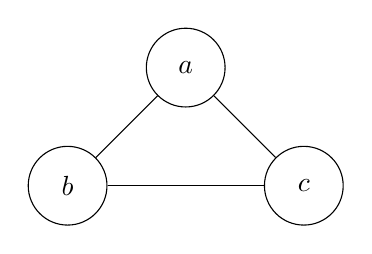
\begin{tikzpicture}[scale=1.5, every node/.style={draw, circle, minimum size=1cm, inner sep=0pt}]
            % Define the nodes for the first graph
            \node (a) at (2,1) {$a$};
            \node (b) at (1,0) {$b$};
            \node (c) at (3,0) {$c$};

            % Draw edges
            \draw (a) -- (b);
            \draw (b) -- (c);
            \draw (c) -- (a);
        \end{tikzpicture}
    \end{center}

    The graph has a dominating set of size $1$, for example, $D = \set{a}$ is a dominating set because $a \in D$ and both $b$ and $c$ are connected to $a$. 

    Notice the difference between a dominating set and a vertex cover: In the graph above, $D = \set{a}$ is \emph{not} a vertex cover because it does not cover the edge $(b,c)$. However, $C = \set{b,c}$ is both a vertex cover and a dominating set. 

    Let $G$ be an undirected graph and $k$ be a nonnegative integer. Consider the following language:
    \[
        \DomSet = \set{(G,k) = \text{$G$ has a dominating set of size (at most) $k$}}.
    \]

    In this problem, you will show that $\DomSet$ is \NP-complete.

  \begin{parts}
      \part [6] Prove that $\DomSet \in \NP$. Specifically, you need to 
              \begin{enumerate}[(i)]
                \item define a certificate\footnote{By ``defining a certificate," we mean describing the \emph{data type} of the certificate. For example, the certificate may be an array, a set, a graph, etc. You may define it in the ``Input" section of the algorithm, similar to $\Upsilon$'s and $\Lambda$'s verifiers in \cref{Upsilon-verifiers}. You should not require the certificate to satisfy any criteria that would trivialize its validity.} and argue that it is polynomial in size with respect to the instance\footnote{The specific polynomial can depend on the verifier, but the same polynomial bounds the certificate size for \emph{all} instances of the language.},
                  \item give an efficient verifier for the language that takes in an instance and a certificate as input, 
                  \item give a correctness argument for the verifier, and
                  \item give a runtime analysis for the verifier.
              \end{enumerate}
              In your verifier, you may assume that the certificate is well-formed, so you do not have to check for it's \emph{data type} (e.g., a graph), but you still have to check for its \emph{validity}.\label{dom-set-np}

              \begin{solution} 
              \begin{enumerate}[label=(\roman*)]
              \item A suitable certificate is a set of vertices \(D \subseteq V\) with \(\lvert D \rvert \le k\). This set can be encoded using a list of vertex identifiers, which is of size polynomial in the size of the input.

              \item The verifier takes as input \((G,k)\) and the certificate \(D\). It checks that \(\lvert D \rvert \le k\). Then, for each vertex \(v \in V\), it checks whether \(v \in D\) or there is an edge from \(v\) to some \(u \in D\). If all vertices satisfy this property, the verifier accepts; otherwise, it rejects.
              
              \item If there is a dominating set of size at most \(k\), then providing that set as a certificate causes the verifier to accept. If there is no dominating set of size at most \(k\), then no certificate can pass the verifier’s checks.
              
              \item Checking, for each \(v\), whether there is an edge to some \(u \in D\) can be done in polynomial time by scanning adjacency lists or an adjacency matrix. Hence, the verification runs in polynomial time.
              \end{enumerate}
              \end{solution}

        \part [4] Since $\DomSet$ has some resemblance to $\VC$, a good source of inspiration is the $\TSAT \ptimemap \VC$ reduction from lecture. 

        We modify the reduction as follows: Given a $\TSAT$ instance (a 3CNF formula) $\phi$, we output~$f(\phi) = (G,k)$ where the ``budget'' $k=n$ is the number of variables in~$\phi$, and graph~$G$ is constructed as follows.
    \begin{itemize}
    \item For each variable $x_i$ in~$\phi$ we create a ``variable gadget'' consisting of \textbf{four} vertices labeled $T_i$ (for true), $F_i$ (for false), $\alpha_i$, and $\beta_i$, along with edges $(T_i,F_i)$, $(\alpha_i, T_i)$, $(\alpha_i, F_i)$, $(\beta_i, T_i)$, and $(\beta_i, F_i)$.
    \item For each clause $C_j$ in $\phi$ we create a \textbf{single} vertex labeled $C_j$, and introduce an edge between $C_j$ and $T_i$ if the literal $x_i$ appears in $C_j$, and an edge between $C_j$ and $F_i$ if the literal $\overline{x_i}$ appears in $C_j$.
    \end{itemize} 

    This reduction is correct, which you will prove in \cref{dom-set-proof}.

    Now, consider the following ``yes" instance in $\TSAT$:
    \[
        \phi = (x_1 \lor \overline x_2 \lor x_3) \land (\overline x_1 \lor x_2 \lor \overline x_3) \land (\overline x_1 \lor \overline x_2 \lor x_3) \land (\overline x_1 \lor \overline x_2 \lor \overline x_3)
    \]

    Determine $f(\phi) = (G,k)$, i.e., give the graph output by the reduction given $\phi$ and specify what $k$ should be. Then, show that $\phi \in \TSAT$ by giving \emph{a} dominating set of $G$ that has (at most) $k$ vertices (if there are multiple, just give any \emph{one} of them). 

    
    \label{dom-set-reduction}
 

        \begin{solution}
        \(\;k = 3\). For each variable \(x_i\), create four vertices \(T_i, F_i, \alpha_i, \beta_i\) with edges
        \[
        (T_i,F_i),\; (\alpha_i,T_i),\; (\alpha_i,F_i),\; (\beta_i,T_i),\; (\beta_i,F_i).
        \]
        For each clause \(C_j\), create a single vertex labeled \(C_j\) and add edges from \(C_j\) to \(T_i\) if \(x_i\) appears in \(C_j\), and from \(C_j\) to \(F_i\) if \(\overline{x_i}\) appears in \(C_j\). Here, this looks like:
        \[
        C_1 \text{ connects to } T_1,\,F_2,\,T_3,\quad
        C_2 \text{ connects to } F_1,\,T_2,\,F_3,
        \]
        \[
        C_3 \text{ connects to } F_1,\,F_2,\,T_3,\quad
        C_4 \text{ connects to } F_1,\,F_2,\,F_3.
        \]
        To show that $\phi \in \TSAT$, an assignment for \(\phi\) is \(x_1 = \text{false},\; x_2 = \text{false},\; x_3 = \text{true}\).
        \[
        D = \{\,F_1,\;F_2,\;T_3\}.
        \]
        Each variable gadget is dominated because \(\alpha_i\) and \(\beta_i\) connect to both \(T_i\) and \(F_i\), and each clause vertex \(C_j\) has an edge to at least one chosen \(T_i\) or \(F_i\). \(D\) is a dominating set of size at most \(k=3\).
        \end{solution}

        \part [8] Prove that the reduction in \cref{dom-set-reduction} is correct, i.e., show that 
        \[
            \phi \in \TSAT \iff f(\phi) = (G,k) \in \DomSet.
        \]
        Moreover, the reduction takes polynomial time in the size of the input formula, because it creates $O(1)$ vertices and edges per vertex and clause. Since $\TSAT$ is \NP-hard, we can conclude that $\DomSet$ is \NP-hard. \label{dom-set-proof}

        \begin{solution}
        \begin{itemize}
        \item \emph{Forward direction:} If \(\phi\) is satisfiable, for each variable \(x_i\), if \(x_i=\text{true}\), pick the vertex \(T_i\). Otherwise, pick \(F_i\) (if \(x_i=\text{false}\)). This set has size equal to the number of variables and dominates all clause vertices (each clause connects to a satisfied literal) as well as all vertices \(\alpha_i,\beta_i\).
        
        \item \emph{Reverse direction:} If there is a dominating set of size \(k\) in \(G\), at most one vertex among \(\{\alpha_i,\beta_i\}\) can dominate those vertices, so each variable gadget must include exactly one of \(T_i\) or \(F_i\). This induces a satisfying assignment for \(\phi\): setting \(x_i=\text{true}\) if \(T_i\in\) the dominating set and \(x_i=\text{false}\) if \(F_i\in\) the dominating set. Since each clause vertex is dominated by one of the chosen \(T_i\) or \(F_i\), every clause has a satisfied literal.
        
        \item The graph has \(O(n)\) vertices from variables plus \(O(m)\) vertices from clauses (where \(n\) is the number of variables and \(m\) is the number of clauses). Each edge is added in constant time per literal. Hence the construction is polynomial in the size of \(\phi\).
        \end{itemize}
        Since \(\TSAT\) is \NP-hard, it follows that \(\DomSet\) is \NP-hard.
        \end{solution}
  \end{parts}
  \pagebreak

  \question \textbf{Subgraph isomorphism.} \label{subgraphiso}
  
For two graphs $G = (V,E)$ and $H = (W, F)$, an \emph{isomorphism} between them is a \emph{bijection} $f:V \to W$ such that $(u,v) \in E$ if and only if $(f(u), f(v)) \in F$. Two graphs are said to be \emph{isomorphic} if there exists an isomorphism between them. For example, the following two graphs are isomorphic, by the bijection $f$ where $f(1) = 1$, $f(2) = 3$, $f(3) = 5$, $f(4) = 2$, and $f(5) = 4$. 

\begin{figure}[H]
    \centering
    \begin{minipage}{0.45\textwidth}
        \centering
        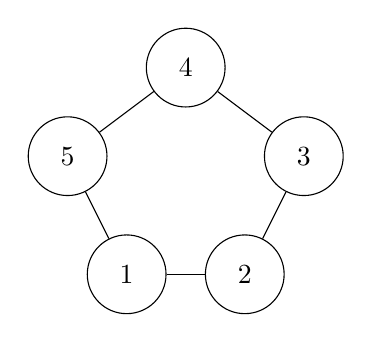
\begin{tikzpicture}[scale=1.5, every node/.style={draw, circle, minimum size=1cm, inner sep=0pt}]
            % Define the nodes for the first graph
            \node (1) at (1,0) {$1$};
            \node (2) at (2,0) {$2$};
            \node (3) at (2.5,1) {$3$};
            \node (4) at (1.5,1.75) {$4$};
            \node (5) at (0.5,1) {$5$};

            % Draw edges
            \draw (1) -- (2);
            \draw (2) -- (3);
            \draw (3) -- (4);
            \draw (4) -- (5);
            \draw (5) -- (1);
        \end{tikzpicture}
    \end{minipage}
    \begin{minipage}{0.45\textwidth}
        \centering
        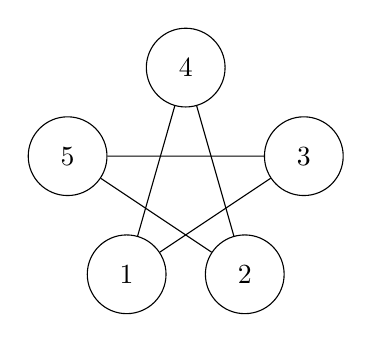
\begin{tikzpicture}[scale=1.5, every node/.style={draw, circle, minimum size=1cm, inner sep=0pt}]
            \node (1') at (1,0) {$1$};
            \node (2') at (2,0) {$2$};
            \node (3') at (2.5,1) {$3$};
            \node (4') at (1.5,1.75) {$4$};
            \node (5') at (0.5,1) {$5$};

            \draw (1') -- (4');
            \draw (2') -- (4');
            \draw (2') -- (5');
            \draw (5') -- (3');
            \draw (3') -- (1');
        \end{tikzpicture}
    \end{minipage}
\end{figure}

     Recall that a subgraph $G' = (V', E')$ of $G = (V, E)$ is a graph such that $V' \subseteq V$ and $E' \subseteq E$. Let $G$ and $H$ be undirected graphs. Consider the following language
      \newcommand{\subgraphiso}{\textsc{Subgraph-Isomorphism}}
      \[
        \subgraphiso = \set{(\inner{G}, \inner{H}): \text{$G$ has a subgraph $G'$ that is isomorphic to $H$}}.
      \]

      In this problem, we will prove that $\subgraphiso$ is \NP-complete.

        \begin{parts}
            \part [6] Prove that $\subgraphiso \in \NP$. Remember to include all steps as in \cref{dom-set} \cref{dom-set-np}.
            
            \begin{solution} 
            \begin{enumerate}[label=(\roman*)]
              \item Let the instance be $(G,H)$, with $G=(V,E)$ and $H=(W,F)$. A valid certificate can be specified by a function $f: W \rightarrow V$, represented as a list of vertex images $\bigl(f(w_1), f(w_2), \dots, f(w_{|W|})\bigr)$. This certificate has size polynomial in $|V|$ and $|W|$.
          
              \item Given $(G,H)$ and the certificate $f$, the verifier performs the following checks:
              \begin{enumerate}
                  \item Ensure that $f$ is injective; that is, no two distinct vertices of $W$ map to the same vertex of $V$.
                  \item For every edge $(w_i,w_j)\in F$, check that $\bigl(f(w_i), f(w_j)\bigr)\in E$. 
                  \item For every non-edge $(w_i, w_j)\notin F$, check that $\bigl(f(w_i), f(w_j)\bigr)\notin E$ if subgraph isolation requires preserving the absence of edges among only those vertices in the induced subgraph on $f(W)$. (Alternatively, it suffices to check edge preservation if the definition of subgraph isomorphism does not require completeness of non-edges. Standard definitions typically only require adjacency preservation, so many presentations omit this step.)
              \end{enumerate}
          
              \item
              \begin{itemize}
                  \item If $G$ contains a subgraph isomorphic to $H$, there exists an injective mapping $f$ that preserves adjacency. This mapping will pass the verifier’s checks.
                  \item If no such subgraph exists, no certificate $f$ can satisfy all adjacency requirements.
              \end{itemize}
          
              \item Checking injectivity can be done in $O(|W|)$ time by recording used vertices in $V$. Checking all edges in $F$ against $E$ is $O(|F|)$. All these steps run in polynomial time in the sizes of $G$ and $H$. Hence the verifier runs in polynomial time.
            \end{enumerate}
            \end{solution}
            
            \part [12] Prove that $\CLIQUE \ptimemap \subgraphiso$. Specifically, you need to 
            \begin{enumerate}[(i)]
                \item give a PTMR from $\CLIQUE$ to $\subgraphiso$,
                \item give a correctness argument for the reduction, and
                \item give a runtime analysis for the reduction.
            \end{enumerate}
            Since $\CLIQUE$ is \NP-hard, we can conclude that $\subgraphiso$ is \NP-hard. 

            \hint{Consider different ranges of $k$ in relation to $|V|$.} \label{subgraphiso-ptmr}
            
            \begin{solution} 
            \begin{enumerate}[label=(\roman*)]
              \item Let $(G,k)$ be an instance of the $\CLIQUE$ problem, where $G=(V,E)$. Construct an instance $\bigl(G, K_k\bigr)$ of $\subgraphiso$, where $K_k$ is the complete graph on $k$ vertices.
          
              \item 
              \begin{itemize}
                  \item ($\Rightarrow$) If $G$ contains a $k$-clique, then there is a set of $k$ vertices in $G$ such that all pairs in that set are adjacent. Those $k$ vertices span a subgraph of $G$ isomorphic to $K_k$, so $(G,K_k)$ is a “yes” instance of $\subgraphiso$.
                  \item ($\Leftarrow$) If $(G,K_k)$ is a “yes” instance of $\subgraphiso$, then $G$ has a subgraph on $k$ vertices that is isomorphic to $K_k$. That subgraph corresponds to a clique of size $k$ in $G$.
              \end{itemize}
          
              \item The graph $K_k$ can be constructed in $O(k^2)$ time by adding $k$ vertices and connecting every pair. Incorporating $G$ unchanged is $O(|V|+|E|)$. Hence the entire reduction runs in polynomial time with respect to the size of $(G,k)$.
            
            \end{enumerate}
            Thus, $\CLIQUE \ptimemap \subgraphiso.$ Since $\CLIQUE$ is \NP-hard and $(G,k) \mapsto (G, K_k)$ is a PTMR, $\subgraphiso$ is also \NP-hard.
            \end{solution}
      \end{parts}

      \pagebreak

  \question [8] \textbf{Big independent sets.} 

  Recall that an \emph{independent set} of an undirected graph $G=(V,E)$ is a subset $I \subseteq V$ such that no two (distinct) vertices in~$I$ have an edge between them.

  In lecture, we proved that the following language is \NP-complete.
  \[
    \IS = \set{(G,k) : G = (V,E) \text{ has an independent set of size (at least) } k} .
  \]

  In this problem, we will explore the following variant of $\IS$. 

    \newcommand{\BigIS}{\textsc{BIG-IS}}
    \[
      \BigIS = \set{ G : G=(V,E) \text{ has an independent set of size (at least) } |V|-1 } .
    \]
  
    Either prove that $\BigIS\in \P$ (by giving a polynomial-time algorithm that decides $\BigIS$) or that $\BigIS$ is $\NP$-hard (by showing that $\IS \ptimemap \BigIS$). If you are giving a reduction, remember to include all steps as in \cref{subgraphiso} \cref{subgraphiso-ptmr}.
    
    \begin{solution}
    \(\BigIS \in \P.\) Let \(G=(V,E)\) be an input graph. The following algorithm decides whether \(G \in \BigIS\) in polynomial time:
    
    \begin{enumerate}
      \item If \(E = \emptyset\), accept, because \(\lvert V \rvert\) vertices form an independent set.
      \item Otherwise, pick any edge \((u,v) \in E\).
      \item Check whether every edge in \(E\) is incident on \(u\). If so, accept.
      \item Check whether every edge in \(E\) is incident on \(v\). If so, accept.
      \item Otherwise, reject.
    \end{enumerate}
    
    Correctness follows from the observation that a graph admits an independent set of size \(\lvert V \rvert - 1\) exactly when there is at most one vertex that all edges share as an endpoint. If there are two such vertices, then they are adjacent, and the independent set cannot include both.  If there are no such vertices, then all vertices are independent. If there are more than two, the algorithm correctly rejects.

    The runtime of the algorithm is polynomial in \(\lvert V \rvert + \lvert E \rvert\). 
    
    \(\BigIS \in \P.\)
    \end{solution}

\end{questions}

\end{document}
